%%%%%%%%%%%%%%%%%%%%%%%%%%%%%%%%%%%%%%%%%%%%%%%%%%%%%%%%%%%%%%%%%%%%%%%%%%%%%%%
%                       DOCUMENT CLASS AND PACKAGES                         %
%%%%%%%%%%%%%%%%%%%%%%%%%%%%%%%%%%%%%%%%%%%%%%%%%%%%%%%%%%%%%%%%%%%%%%%%%%%%%%%

\documentclass[11pt,english]{report}


\usepackage[utf8]{inputenc} 


\usepackage{graphicx} 

\usepackage[english]{babel}
\usepackage{amsmath} 
\usepackage{booktabs} 
\usepackage{multirow}
\usepackage{float}
\usepackage{array} % Added for p{} column type
\usepackage{tikz}
\usetikzlibrary{positioning, arrows.meta, calc, backgrounds, fit, shapes.geometric, matrix, chains}
\usepackage{pgfplots}
\pgfplotsset{compat=1.18}
\usepgfplotslibrary{groupplots}
\usepackage{natbib}            
\usepackage{pdfpages}
\usepackage{parskip}
\usepackage{tabularx} % put this in your preamble

\setlength{\parindent}{0pt}
\setlength{\parskip}{1em} 

%%%%%%%%%%%%%%%%%%%%%%%%%%%%%%%%%%%%%%%%%%%%%%%%%%%%%%%%%%%%%%%%%%%%%%%%%%%%%%%
%                 INFORMATION FOR THE COVER PAGE AND DOCUMENT               %
%          (Fill in or modify the fields as necessary)                      %
%%%%%%%%%%%%%%%%%%%%%%%%%%%%%%%%%%%%%%%%%%%%%%%%%%%%%%%%%%%%%%%%%%%%%%%%%%%%%%%

\newcommand{\theuniversity}{Universitat Politècnica de València}
\newcommand{\theschool}{DSIC - Departament de Sistemes Informàtics i Computació}
\newcommand{\thedegree}{MIARFID - Master's in Artificial Intelligence and Pattern Recognition}
\newcommand{\theprojecttype}{Academic Project}

\newcommand{\thetitle}{Optimization of Keyboard Layouts for English}
\newcommand{\theauthor}{Jordi Cantavella Ferrero}
\newcommand{\thecourse}{Academic Year 2025-2026}


%%%%%%%%%%%%%%%%%%%%%%%%%%%%%%%%%%%%%%%%%%%%%%%%%%%%%%%%%%%%%%%%%%%%%%%%%%%%%%%
%                              START OF DOCUMENT                              %
%%%%%%%%%%%%%%%%%%%%%%%%%%%%%%%%%%%%%%%%%%%%%%%%%%%%%%%%%%%%%%%%%%%%%%%%%%%%%%%
\usepackage[colorlinks=true, linkcolor=purple, citecolor=green!60!black, urlcolor=magenta]{hyperref}

\begin{document}

\begin{titlepage}
    \centering
    
    \vspace{1.5cm}
    
    {\Large \bfseries \theuniversity} \\
    \vspace{0.5cm}
    {\large \theschool} \\
    
    \vspace{2cm}
    
    {\large \textbf{\theprojecttype}} \\
    \vspace{0.2cm}
    {\large \thedegree} \\
    
    \vfill 
    
    {\Huge \bfseries \thetitle} \\
    
    \vfill
    
    \begin{minipage}{0.8\textwidth}
        \begin{flushleft}
            \large
            \textbf{Author:} \\
            \theauthor \\
            \vspace{1cm}
        \end{flushleft}
    \end{minipage}
    
    \vfill
    
    {\large \thecourse}
    
\end{titlepage}


\tableofcontents
\listoffigures
\listoftables
\cleardoublepage

%%%%%%%%%%%%%%%%%%%%%%%%%%%%%%%%%%%%%%%%%%%%%%%%%%%%%%%%%%%%%%%%%%%%%%%%%%%%%%%
%                    MAIN CONTENT STRUCTURE                                 %
%%%%%%%%%%%%%%%%%%%%%%%%%%%%%%%%%%%%%%%%%%%%%%%%%%%%%%%%%%%%%%%%%%%%%%%%%%%%%%%

\chapter{Introduction} \label{chpt:1}
\section{Context}
The layout of current keyboards is not optimized for ergonomics and typing efficiency. 
Current layouts have their roots in traditional typewriting and have not evolved to meet the modern needs of users.
Layouts like QWERTY, which emerged in 1873, were designed for mechanical typewriters and are no longer the most efficient for typing on digital devices.

Later studies showed that the QWERTY layout generated inefficient movements, contributing to fatigue and the risk of injury.
This led to subsequent layouts such as Dvorak (1936) and Colemak (2006), which aimed to improve efficiency and reduce user fatigue.
Seeking to maximize typing speed and minimize physical effort, these layouts are based on ergonomic principles and linguistic analysis.

\section{Objectives}
The main objective of this work is the optimization of keyboard layouts, aiming to generate ergonomic and efficient keyboard arrangements.
To achieve this, a genetic algorithm and simulated annealing will be implemented to explore the space of possible layouts and find optimal configurations
based on ergonomic and linguistic criteria.
\begin{itemize}
    \item Implement a genetic algorithm for generating and evaluating different keyboard layouts.
    \item Implement a simulated annealing algorithm for the same problem.
    \item Define evaluation metrics that consider distance, hand alternation, and finger effort.
    \item Analyze the results obtained by the algorithms.
    \item Compare the generated layouts with existing ones such as \textit{QWERTY}, \textit{Dvorak}, and \textit{Colemak}.
\end{itemize}

\section{Scope and Limitations}
Given the time and resource constraints, this work will focus on optimizing keyboard layouts for the English language.
Aspects related to the physical implementation of keyboards or adaptation to different devices will not be addressed.

Also given the different characteristiscs of each distribution, the optimization will be focused on the most common Latin alphabet layouts,
including all the letteres, and the most common punctuation marks.

\chapter{Theoretical Framework} \label{chpt:2}
\section{History of Keyboard Layouts} \label{sec:historia_teclados}
Over time, different types of keyboards have been used, from the first mechanical keyboards to modern digital ones.
Among them, the QWERTY, Dvorak, and Colemak keyboards have been particularly prominent.

The \textbf{QWERTY} keyboard, designed in 1873 by Christopher Latham Sholes, was created to prevent the keys of early mechanical typewriters from jamming.
Its design prioritized separating the most frequently used letters in English to reduce typing speed and prevent the typebars from clashing.

The \textbf{Dvorak} keyboard, developed in 1936 by August Dvorak and his brother-in-law William Dealey, was designed to improve efficiency and reduce user fatigue.
It demonstrated a reduction of up to 35\% in finger movement compared to the QWERTY layout by placing the most used letters on the home row and promoting hand alternation.

The \textbf{Colemak} keyboard, introduced in 2006 by Shai Coleman, is an evolution of the QWERTY keyboard that aims to improve efficiency without requiring a radical change in key arrangement.
Colemak keeps many keys in their original positions, making the transition easier for users accustomed to QWERTY.
It focuses on minimizing finger movement and maximizing typing speed by placing the most common letters in accessible positions.

As shown in Figure \ref{fig:keyboard_layouts}, each of these layouts takes a different approach to ergonomics and efficiency, reflecting the needs and technologies of its time.

\begin{figure}[H]
    \centering
    \includegraphics[width=0.7\textwidth]{images/qwerty-dvorak-colemak.jpg}
    \caption{Comparison of the QWERTY, Dvorak, and Colemak keyboard layouts.}
    \label{fig:keyboard_layouts}

\end{figure}

Representing the different keyboard layouts, Figure \ref{fig:keyboard_layouts} illustrates how each of these arrangements seeks to optimize the typing experience from different perspectives.
Note the concentration of the most used letters on the home row of the Dvorak and Colemak keyboards, in contrast to the more scattered arrangement of the QWERTY keyboard.

\section{Keyboard Ergonomics} \label{sec:ergonomia_teclado}
Following the main layouts introduced in section \ref{sec:historia_teclados}, keyboard ergonomics is a crucial aspect in the design of keyboard layouts.
The hand has a series of anatomical characteristics that influence comfort and efficiency when typing. Among them, we highlight:
\begin{itemize}
    \item \textbf{Finger Strength:} The strength of the fingers varies, with the thumb and middle finger being the strongest, while the pinky is the weakest.
    \item \textbf{Finger Mobility:} Fingers have different ranges of motion, with the thumb and index finger being the most mobile.
    \item \textbf{Muscle Fatigue:} Prolonged use of certain fingers can lead to muscle fatigue, especially if constant effort is required.
    \item \textbf{Hand Posture:} A natural and relaxed hand posture is essential to avoid strain and long-term injuries.
\end{itemize}

\section{Linguistic Analysis} \label{sec:analisis_linguistico}
Linguistic analysis is fundamental for designing keyboard layouts that optimize typing efficiency.
Paying attention to the frequency of letters and their distribution will allow us to design keyboards that minimize finger movement and maximize typing speed.

Figure \ref{fig:english_letter_frequency} shows an analysis of letter frequency in English.

\begin{figure}[H]
    \centering
    \includegraphics[width=0.8\textwidth]{images/english.png}
    \caption{Frequency of letters in English.}
    \label{fig:english_letter_frequency}
\end{figure}



Figure \ref{fig:letter_frequency_languages} shows the frequency distribution of the 26 most common letters used in Latin-based alphabets,
covering all languages that use the Latin alphabet, such as Spanish, English, French, German, and Italian.
It can be observed that the frequency of letters varies among different languages, which influences the optimal design of keyboard layouts for each language,
even though these languages share a similar alphabet and common origin.

\begin{figure}[H]
    \centering
    \includegraphics[width=1\textwidth]{images/idiomas.png}
    \caption{Frequency of letters in different languages.}
    \label{fig:letter_frequency_languages}
\end{figure}

As observed in Figure \ref{fig:letter_frequency_languages}, the frequency varies across different languages.
It is also important to note that our reference corpus must capture a diverse range of language use, including formal and informal texts, to obtain an accurate representation of the frequency 
of letters and letter combinations.

\section{Used datasets} \label{sec:datasets}
In order to analyse the different types of texts and their characteristics, this works uses different types of books or texts as their testing datasets.
For a more classical literature approach, we have used \textit{Moby Dick} by Herman Melville, a classic work of English literature. 
This novel provides a rich and varied vocabulary, making it suitable for analyzing letter and bigram frequencies in traditional literary texts.

Representing a simpler style, we use \textit{The Wonderful Wizard of Oz} by L. Frank Baum. This book features a more constrained and common vocabulary, simpler sentence structures, 
and repetitive phrasing typical of children's literature. A layout optimized for this corpus should reflect the patterns of more common, everyday English usage.


For each corpus, the raw text will be pre-processed to normalize the data: all letters will be converted to lowercase, and all punctuation except the used in the algorithms, numbers, 
and whitespace will be removed. From the resulting continuous stream of characters, we will compute the fitness of each individual in order to determine how good they are 
as a keyboard layout.

\chapter{Genetic Algorithm Methodology} \label{chpt:3}
This section describes the methodology used to implement a genetic algorithm for optimizing keyboard layouts.


\section{Problem Modeling} \label{sec:modelado_problema}
The keyboard layout optimization problem can be modeled as a combinatorial optimization problem where the goal is to find the best arrangement of keys on a keyboard.
In our particular case, we will focus on the 26 letters of the English alphabet and a few punctuation marks. Trying to minimize the fitness function later introduced in section \ref{sec:funcion_evaluacion}.
Each keyboard layout can be represented as a permutation of the set of characters to be arranged on the keyboard.
Our considered set of letters and symbols includes the 26 letters of the English alphabet, along with the space character, period (.), comma (,), semicolon (:) and apostrophe (').

To model our individuals, we use a list of characters where each position corresponds to a specific key on the keyboard. The keyboard is divided into three rows and ten columns, 
giving us a total of 30 positions that will be filled with the characters from our set. Each key can only be occupied by one character, and each character can only appear once 
in the layout, ensuring that each individual represents a valid permutation.

The keyboard layout is represented as a standard 3 X 10 grid structure:
\begin{center} 
    \begin{verbatim}
        0,  1,  2,  3,  4,  5,  6,  7,  8,  9
        10, 11, 12, 13, 14, 15, 16, 17, 18, 19
        20, 21, 22, 23, 24, 25, 26, 27, 28, 29
    \end{verbatim}
\end{center}

Each position is assigned to a specific finger based on standard touch typing conventions, with finger assignments considering hand (left/right), 
finger type (pinky, ring, middle, index), and relative strength values.

\begin{figure}[htbp]
\centering

% Define colors for each finger
\definecolor{finger0}{RGB}{255, 99, 71}
\definecolor{finger1}{RGB}{255, 165, 0}
\definecolor{finger2}{RGB}{255, 215, 0}
\definecolor{finger3}{RGB}{50, 205, 50}

\begin{tikzpicture}[scale=0.7]
    
    % Title
    \node at (5, 3.5) {\texttt{Finger Mapping Grid (3×10)}};
    
    % LEFT HAND LABEL
    \node at (2, 2.7) {\textbf{LEFT}};
    
    % Left Hand (columns 0-4)
    % Row 2 (top) - ahora empieza en 0
    \fill[finger0] (0, 2) rectangle (1, 3);
    \node[white] at (0.5, 2.5) {0};
    \fill[finger1] (1, 2) rectangle (2, 3);
    \node[white] at (1.5, 2.5) {1};
    \fill[finger2] (2, 2) rectangle (3, 3);
    \node[white] at (2.5, 2.5) {2};
    \fill[finger3] (3, 2) rectangle (4, 3);
    \node[white] at (3.5, 2.5) {3};
    \fill[finger3] (4, 2) rectangle (5, 3);
    \node[white] at (4.5, 2.5) {4};
    
    % Row 1 (middle)
    \fill[finger0] (0, 1) rectangle (1, 2);
    \node[white] at (0.5, 1.5) {10};
    \fill[finger1] (1, 1) rectangle (2, 2);
    \node[white] at (1.5, 1.5) {11};
    \fill[finger2] (2, 1) rectangle (3, 2);
    \node[white] at (2.5, 1.5) {12};
    \fill[finger3] (3, 1) rectangle (4, 2);
    \node[white] at (3.5, 1.5) {13};
    \fill[finger3] (4, 1) rectangle (5, 2);
    \node[white] at (4.5, 1.5) {14};
    
    % Row 0 (bottom)
    \fill[finger0] (0, 0) rectangle (1, 1);
    \node[white] at (0.5, 0.5) {20};
    \fill[finger1] (1, 0) rectangle (2, 1);
    \node[white] at (1.5, 0.5) {21};
    \fill[finger2] (2, 0) rectangle (3, 1);
    \node[white] at (2.5, 0.5) {22};
    \fill[finger3] (3, 0) rectangle (4, 1);
    \node[white] at (3.5, 0.5) {23};
    \fill[finger3] (4, 0) rectangle (5, 1);
    \node[white] at (4.5, 0.5) {24};
    
    % Draw left hand grid
    \draw[very thick] (0, 0) rectangle (5, 3);
    \foreach \x in {1,2,3,4} \draw[thick] (\x, 0) -- (\x, 3);
    \foreach \y in {1,2} \draw[thick] (0, \y) -- (5, \y);
    
    % DIVIDER
    \fill[gray!70] (5.15, -0.1) rectangle (5.35, 3.1);
    
    % RIGHT HAND LABEL
    \node at (7.75, 2.7) {\textbf{RIGHT}};
    
    % Right Hand (columns 5-9)
    % Row 2 (top)
    \fill[finger3] (5.5, 2) rectangle (6.5, 3);
    \node[white] at (6, 2.5) {5};
    \fill[finger3] (6.5, 2) rectangle (7.5, 3);
    \node[white] at (7, 2.5) {6};
    \fill[finger2] (7.5, 2) rectangle (8.5, 3);
    \node[white] at (8, 2.5) {7};
    \fill[finger1] (8.5, 2) rectangle (9.5, 3);
    \node[white] at (9, 2.5) {8};
    \fill[finger0] (9.5, 2) rectangle (10.5, 3);
    \node[white] at (10, 2.5) {9};
    
    % Row 1 (middle)
    \fill[finger3] (5.5, 1) rectangle (6.5, 2);
    \node[white] at (6, 1.5) {15};
    \fill[finger3] (6.5, 1) rectangle (7.5, 2);
    \node[white] at (7, 1.5) {16};
    \fill[finger2] (7.5, 1) rectangle (8.5, 2);
    \node[white] at (8, 1.5) {17};
    \fill[finger1] (8.5, 1) rectangle (9.5, 2);
    \node[white] at (9, 1.5) {18};
    \fill[finger0] (9.5, 1) rectangle (10.5, 2);
    \node[white] at (10, 1.5) {19};
    
    % Row 0 (bottom)
    \fill[finger3] (5.5, 0) rectangle (6.5, 1);
    \node[white] at (6, 0.5) {25};
    \fill[finger3] (6.5, 0) rectangle (7.5, 1);
    \node[white] at (7, 0.5) {26};
    \fill[finger2] (7.5, 0) rectangle (8.5, 1);
    \node[white] at (8, 0.5) {27};
    \fill[finger1] (8.5, 0) rectangle (9.5, 1);
    \node[white] at (9, 0.5) {28};
    \fill[finger0] (9.5, 0) rectangle (10.5, 1);
    \node[white] at (10, 0.5) {29};
    
    % Draw right hand grid
    \draw[very thick] (5.5, 0) rectangle (10.5, 3);
    \foreach \x in {6.5,7.5,8.5,9.5} \draw[thick] (\x, 0) -- (\x, 3);
    \foreach \y in {1,2} \draw[thick] (5.5, \y) -- (10.5, \y);
    
    % LEGEND
    \node[left] at (0, -1.15) {\textbf{Legend:}};
    
    \fill[finger0] (1, -0.9) rectangle (1.5, -1.4);
    \node[right] at (1.6, -1.15) {Pinky};
    
    \fill[finger1] (3.8, -0.9) rectangle (4.3, -1.4);
    \node[right] at (4.4, -1.15) {Ring};
    
    \fill[finger2] (6.6, -0.9) rectangle (7.1, -1.4);
    \node[right] at (7.2, -1.15) {Middle};
    
    \fill[finger3] (9.6, -0.9) rectangle (10.1, -1.4);
    \node[right] at (10.2, -1.15) {Index};
    
\end{tikzpicture}

\caption{Finger mapping visualization showing key-to-finger assignments for left and right hands in a 3×10 grid.}
\label{fig:finger_mapping}
\end{figure}

\section{Initial Population} \label{sec:poblacion_inicial}
The initial population is created by combining well knowon existing layouts with randomly generated layouts, providing the genetetic a good starting point for exploration.
The \texttt{init\_population} function generates a specified number of individuals, each representing a different keyboard layout, using the following approach:
When the \texttt{known\_distributions} parameter is set to True, the algorithm includes four well-established keyboard layouts as part of the initial population:

\begin{itemize}

    \item \texttt{QWERTY}: The most common layout, designed originally for typewriters
    \item \texttt{Dvorak}: Scientifically designed layout focused on efficiency and reduced finger movement
    \item \texttt{QWERTZ}: German variant of QWERTY with Y and Z positions swapped
    \item \texttt{Colemak}: Modern layout designed to improve upon QWERTY while maintaining some key positions
\end{itemize}

The remaining individuals in the population are generated randomly to ensure diversity. This individuals are created by shuffling the list of characters to be arranged on the keyboard, 
ensuring that each layout is a valid permutation of the character set. This hybrid approach of combining known layouts with random enables the genetic algorithm to start with some good
solutions while also exploring a wide range of possibilities.

Each individual in the population undergoes validation to ensure it contains exactly 30 characters with no duplicates or missing characters from the defined character set.


\section{Fitness Function} \label{sec:evaluation_function}
The fitness function evaluates the quality of a keyboard layout by calculating the total "typing cost" when typing a given text. Lower fitness scores indicate better layouts. 
The function considers multiple factors that affect typing efficiency and ergonomics.

For each consecutive pair of characters in the input text, the algorithm calculates:
\begin{enumerate}
    \item \texttt{Euclidean distance:} the geometric distance between key positions on the 3×10 grid
    \item \texttt{Finger penalty:} additional costs based on ergonomic factors
\end{enumerate}


The \texttt{finger\_penalty} function implements a comprehensive penalty system based on:
\begin{itemize}
    \item \texttt{Same Finger Usage:} heavy penalty (1.0) when consecutive characters require the same finger, with additional penalty (2.0) for weak fingers (pinky and ring finger).
    \item \texttt{Same Hand Usage:} moderate penalty (1.0) when both characters are typed with the same hand, promoting hand alternation.

\end{itemize}

Also additional penalties for the vertical movements:
\begin{itemize}
    \item \texttt{Adjacents rows (distance 1):} penalty of 0.2, with additional 0.15 for weak fingers
    \item \texttt{Two-row jumps (distance 2):} Tpenalty of 0.8, with additional 0.5 for weak fingers

\end{itemize}

Regarding the usage of the fingers, the weaker fingers are penalised, based on:
\begin{itemize}
    \item \texttt{Pinky finger usage:} +0.15 penalty
    \item \texttt{Ring finger usage:} +0.1 penalty

\end{itemize}

Finally an additional penalisation for the movements between the same column.
Giving an additional penalty of 0.3 for vertical movement within the same column, 
with extra penalties for outer columns (0.2 for columns 0 and 9, 0.1 for columns 1 and 8).

% So each character pair cost is computed based on:

% \begin{equation}
%     \centering
%     fitness\_function = euclidean\_distance \times \max(1.0 + finger\_penalty, 0.1)
% \end{equation}

% And the objetive is to minimize said fitness functions. 


The cost for each character pair $(c_i, c_{i+1})$ is computed as:

\begin{equation}
    \text{cost}(c_i, c_{i+1}) = d_{\text{euclidean}}(c_i, c_{i+1}) \times \max(1.0 + P_{\text{finger}}(c_i, c_{i+1}), 0.1)
\end{equation}

where $d_{\text{euclidean}}$ represents the Euclidean distance between key positions and $P_{\text{finger}}$ represents the cumulative finger penalty. The total fitness function is then:

\begin{equation}
    F(\mathcal{L}) = \sum_{i=1}^{n-1} \text{cost}(c_i, c_{i+1})
\end{equation}

where $\mathcal{L}$ denotes the keyboard layout, $n$ is the length of the input text, and the objective is to minimize $F(\mathcal{L})$.

\section{New Population Generation} \label{sec:new_population}

\subsection{Selection} \label{sec:selection}
The algorithm implements tournament selection as the primary selection mechanism. The \texttt{tournament\_selection} function works as follows:
\begin{enumerate}
    \item Groups of k elements are established (where k is the size group). In this particular case having k=5 in order to balance between good and bad fitness individuals.
    \item From each group we select the best individual (the one with the lowest fitness function).
    \item We perform successive tournaments to select both parments for the crossover operation.
\end{enumerate}

Using the tournament selection over other selection methods we ensure a good balance between selection pressure and diversity maintenance, allowing both high-quality individuals 
and some lower-quality individuals to participate in reproduction.

\subsection{Crossover} \label{sec:crossover}


To generate new individuals from two parents, the algorithm employs a \textbf{two-point crossover} operator specifically adapted for permutations. 
This method ensures that every child produced is a valid keyboard layout, containing all required characters exactly once. 
The process is executed as follows:

\begin{enumerate}
    \item \texttt{Segment Selection:} two random crossover points are selected along the length of the parent layouts. These points define a central segment.
    \item \texttt{Direct Inheritance:} the child layout inherits this central segment directly from the first parent and the rest from the second.
    \item \texttt{Completion:} fill remaining positions using \texttt{parent2}, applying the mapping to resolve conflicts and ensure valid permutation, based on a reconstruction function.
\end{enumerate}

The crossover operation is applied with a probability of \texttt{crossover\_rate} (set to 0.85). If crossover is not performed, one of the parents is passed directly to the next 
generation, preserving its genetic material without alteration.

A \texttt{fix\_duplicates} function ensures that any potential duplicates are resolved by replacing them with missing characters, maintaining the permutation property.

\subsection{Mutation} \label{sec:mutation}
The mutation operator implements a simple swap mutation strategy:

\begin{enumerate}
    \item \texttt{Mutation detection:} each individual has a probability mutation\_rate = 0.15 of being mutated.
    \item \texttt{Swap Operation:} if mutation occurs, randomly select two positions and swap their characters.
    \item \texttt{Permutation Preservation:} the swap operation maintains the valid permutation property
\end{enumerate}

This mutation strategy provides local search capability while ensuring that all individuals remain valid keyboard layouts.

\subsection{Replacement} \label{sec:replacemnet}
The algorithm uses an elitist replacement strategy that combines the best individuals from the current generation with newly generated offspring:
\begin{enumerate}
    \item \texttt{Elite preservation:} keep the top 50\% of the individuals, particularly elite ones.
    \item \texttt{Offspring integration:} fill the reamining populaton slots with the offspring from corssover and mutation operations.
\end{enumerate}

This approach ensures that good solutions are not lost while allowing new genetic material to enter the population through reproduction operations.
And maintaining a new population the same size as the previous generation.

\section{Experimental setup} \label{sec:experimental_setup}
To evaluate the performance of the genetic algorithm and understand the characteristics of optimized keyboard layouts, 
a series of experiments were designed with varying conditions and corpora.

The baseline configuration used for all experiments is presented in Table \ref{tab:ga_params}. 
These parameters were selected based on preliminary experiments and computational constraints.

\begin{table}[H]
    \centering
    \caption{Genetic Algorithm Hyperparameters}
    \label{tab:ga_params}
    \begin{tabular}{@{}lll@{}}
        \toprule
        \textbf{Parameter} & \textbf{Value} & \textbf{Purpose} \\ 
        \midrule
        Population Size & 10,000 & High diversity \\
        Generations & 100 & Convergence \\
        Elite Size & 1,500 (15\%) & Preserve best solutions \\
        Tournament Size & 5 & Balance pressure/diversity \\
        Crossover Rate & 0.85 & Explore combinations \\
        Mutation Rate & 0.15 & Maintain diversity \\
        Initial Population & Random & Unbiased search \\
        Random seed & 123 & In order to recreate the experiments \\
        \bottomrule
    \end{tabular}
\end{table}


% \subsection{Experimental Design}
% Experiments were conducted over two different corpora, with the objective to obtain and analyze how two different books of two different 
% literary chategories would affect in the generation of an optimal layout.

% To this end we used Moby Dick and Wizard of Oz.


\section{Results and Analysis} \label{sec:results_analysis}

\subsection{Moby Dick Results}

The genetic algorithm was executed on the Moby Dick book with the Hyperparameters specified in the Table \ref{tab:ga_params}.
This classic literary work presents a rich and varied vocabulary, providing a robut test case for keyboard optimization.

Figure \ref{fig:convergence} illustrates the evolutionary progression of the algorithm over 100 generations. 
The fitness function decreased from an initial value of \textbf{1,375,854.6} to a final optimized value of \textbf{799,038.6}, 
representing a 41.9\% improvement through evolution alone.



\begin{figure}[H]
    \centering
    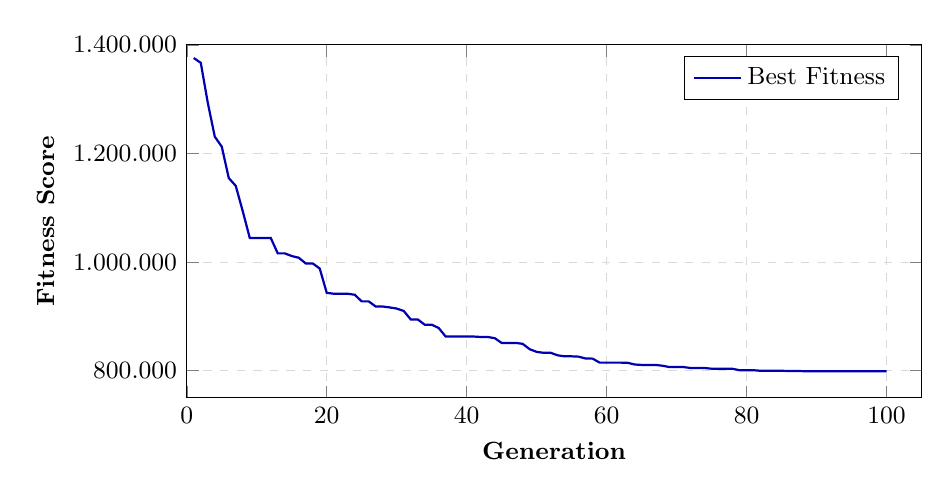
\begin{tikzpicture}
        \begin{axis}[
            width=0.9\textwidth,
            height=0.5\textwidth,
            xlabel={Generation},
            ylabel={Fitness Score},
            grid=major,
            grid style={dashed, gray!30},
            legend pos=north east,
            legend style={font=\small},
            xmin=0, 
            xmax=105,
            ymin=750000, 
            ymax=1400000,
            scaled y ticks=false,
            y tick label style={/pgf/number format/.cd, fixed, precision=0, use comma},
            tick label style={font=\small},
            ylabel style={font=\small\bfseries},
            xlabel style={font=\small\bfseries},
        ]
        
        \addplot[blue!70!black, thick, mark=none] coordinates {
            (1, 1375854.6) (2, 1366983.4) (3, 1293382.1) (4, 1231106.9) (5, 1212478.8)
            (6, 1154810.6) (7, 1140260.0) (8, 1093522.8) (9, 1044380.1) (10, 1044380.1)
            (11, 1044380.1) (12, 1044380.1) (13, 1016003.6) (14, 1016003.6) (15, 1011078.3)
            (16, 1007979.7) (17, 997435.2) (18, 997435.2) (19, 988044.8) (20, 943321.0)
            (21, 941619.3) (22, 941619.3) (23, 941619.3) (24, 939745.2) (25, 927539.3)
            (26, 927539.3) (27, 918065.2) (28, 918065.2) (29, 916432.9) (30, 914313.3)
            (31, 909925.2) (32, 894360.2) (33, 894360.2) (34, 884631.1) (35, 884631.1)
            (36, 878489.3) (37, 862777.3) (38, 862777.3) (39, 862777.3) (40, 862777.3)
            (41, 862777.3) (42, 861987.3) (43, 861987.3) (44, 859766.7) (45, 851063.5)
            (46, 851063.5) (47, 851063.5) (48, 849362.0) (49, 839480.9) (50, 834521.5)
            (51, 832828.8) (52, 832828.8) (53, 828203.3) (54, 826311.0) (55, 826311.0)
            (56, 825731.5) (57, 822289.9) (58, 822099.7) (59, 814739.5) (60, 814739.5)
            (61, 814739.5) (62, 814739.5) (63, 814396.5) (64, 811273.1) (65, 810497.4)
            (66, 810497.4) (67, 810497.4) (68, 808976.6) (69, 806493.9) (70, 806493.9)
            (71, 806493.9) (72, 804826.4) (73, 804826.4) (74, 804826.4) (75, 803519.5)
            (76, 803519.5) (77, 803358.5) (78, 803358.5) (79, 800763.6) (80, 800763.6)
            (81, 800763.6) (82, 799671.8) (83, 799671.8) (84, 799671.8) (85, 799671.8)
            (86, 799348.6) (87, 799348.6) (88, 799038.6) (89, 799038.6) (90, 799038.6)
            (91, 799038.6) (92, 799038.6) (93, 799038.6) (94, 799038.6) (95, 799038.6)
            (96, 799038.6) (97, 799038.6) (98, 799038.6) (99, 799038.6) (100, 799038.6)
        };
        \addlegendentry{Best Fitness}
        
        \end{axis}
    \end{tikzpicture}
    \caption{Genetic algorithm over 100 generations on Moby Dick corpus}
    \label{fig:convergence}
\end{figure}


The convergence pattern exhibits three distinct phases, as detailed in Table \ref{tab:convergence_phases}. 
The initial exploration phase (generations 1-20) shows rapid fitness improvement of 31.4\%, finding new solutions and improving drastically,
during which the algorithm discovers promising keyboard configurations through aggressive exploration of the search space. 
The exploitation phase (generations 21-60) demonstrates more gradual refinement with 13.6\% improvement as the population converges toward 
local optima. Finally, the convergence phase (generations 61-100) shows minimal change (1.9\% improvement), indicating the algorithm has 
reached a stable, high-quality solution.

\begin{table}[H]
    \centering
    \caption{Phhase analysis (Moby dick)}
    \label{tab:convergence_phases}
    \begin{tabularx}{\textwidth}{@{}Xrrrr@{}}
        \toprule
        \textbf{Phase} & \textbf{Generations} & \textbf{Initial Fit.} & \textbf{Final Fit.} & \textbf{Improvement} \\ 
        \midrule
        Exploration  & 1--20   & 1,375,854.6 & 943,321.0   & 31.4\% \\
        Exploitation & 21--60  & 943,321.0   & 814,739.5   & 13.6\% \\
        Convergence  & 61--100 & 814,739.5   & 799,038.6   & 1.9\%  \\
        \midrule
        \textbf{Total} & \textbf{1--100} & \textbf{1,375,854.6} & \textbf{799,038.6} & \textbf{41.9\%} \\
        \bottomrule
    \end{tabularx}
\end{table}

Table \ref{tab:convergence_milestones} presents the fitness evolatuion per decade, showing the descents towards the local optimal solution found.

\begin{table}[H]
    \centering
    \caption{Convergence milestones: Best fitness every 10 generations}
    \label{tab:convergence_milestones}
    \begin{tabular}{@{}rr|rr@{}}
        \toprule
        \textbf{Generation} & \textbf{Best Fitness} & \textbf{Generation} & \textbf{Best Fitness} \\ 
        \midrule
        1  & 1,375,854.6 & 60 & 814,739.5 \\
        10 & 1,044,380.1 & 70 & 806,493.9 \\
        20 & 943,321.0   & 80 & 800,763.6 \\
        30 & 914,313.3   & 90 & 799,038.6 \\
        40 & 862,777.3   & 100 & 799,038.6 \\
        50 & 834,521.5   &     &           \\
        \bottomrule
    \end{tabular}
\end{table}

The result obtaied from this layout represented in Figure \ref{fig:evolved_layout_movie_dick}, shows that the algorithm has distributed
characters across the three rows to minimize typing cost according to the fitness function defined in Section \ref{sec:evaluation_function}.

\begin{figure}[H]
    \centering
    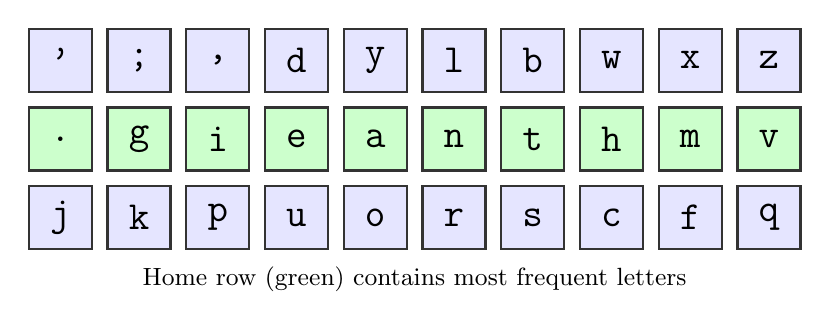
\begin{tikzpicture}[
        key/.style={rectangle, draw=black!80, fill=blue!10, thick, minimum size=0.8cm, font=\Large\ttfamily},
        home/.style={key, fill=green!20},
    ]
    % Row 1
    \node[key] at (0,2) {'}; \node[key] at (1,2) {;}; \node[key] at (2,2) {,}; 
    \node[key] at (3,2) {d}; \node[key] at (4,2) {y}; \node[key] at (5,2) {l}; 
    \node[key] at (6,2) {b}; \node[key] at (7,2) {w}; \node[key] at (8,2) {x}; 
    \node[key] at (9,2) {z};
    
    % Row 2 (Home row - highlighted)
    \node[home] at (0,1) {.}; \node[home] at (1,1) {g}; \node[home] at (2,1) {i}; 
    \node[home] at (3,1) {e}; \node[home] at (4,1) {a}; \node[home] at (5,1) {n}; 
    \node[home] at (6,1) {t}; \node[home] at (7,1) {h}; \node[home] at (8,1) {m}; 
    \node[home] at (9,1) {v};
    
    % Row 3
    \node[key] at (0,0) {j}; \node[key] at (1,0) {k}; \node[key] at (2,0) {p}; 
    \node[key] at (3,0) {u}; \node[key] at (4,0) {o}; \node[key] at (5,0) {r}; 
    \node[key] at (6,0) {s}; \node[key] at (7,0) {c}; \node[key] at (8,0) {f}; 
    \node[key] at (9,0) {q};
    
    \node[below, font=\small] at (4.5, -0.5) {Home row (green) contains most frequent letters};
    \end{tikzpicture}
    \caption{Optimized keyboard layout evolved by genetic algorithm (Moby Dick book)}
    \label{fig:evolved_layout_movie_dick}
\end{figure}

Finally, Table \ref{tab:letter_placement} categorizes the character distribution across rows, revealing the algorithm's 
strategy for minimizing finger movement and maximizing typing efficiency. This distribution aligns with distribution shown in
Figure \ref{fig:english_letter_frequency}, which represents the distribution of the keys.
We can see that the most frequent keys have been placed in the center row or as centered as possible.

\begin{table}[H]
    \centering
    \caption{Letter placement analysis of evolved layout}
    \label{tab:letter_placement}
    \begin{tabularx}{\textwidth}{@{}lX>{\raggedright\arraybackslash}X@{}}
        \toprule
        \textbf{Row} & \textbf{Letters} & \textbf{Notes} \\ 
        \midrule
        Top    & ', ;, ,, d, y, l, b, w, x, z
               & Punctuation and less frequent consonants \\
        Home   & ., g, i, e, a, n, t, h, m, v
               & High-frequency vowels (e, a, i) and consonants (t, n, h) \\
        Bottom & j, k, p, u, o, r, s, c, f, q
               & Mix of vowels (u, o) and common consonants (r, s) \\
        \bottomrule
    \end{tabularx}
\end{table}

To evaluate the effectiveness of the genetic algorithm, the evolved layout was compared against four established keyboard designs: 
QWERTY, QWERTZ, Dvorak, and Colemak. 
All layouts were evaluated using the same fitness function and Moby Dick book to ensure fair comparison.
Table \ref{tab:layout_comparison} presents the fitness scores and percentage improvements of the evolved 
layout over each known layout.


\begin{table}[H]
    \centering
    \caption{Fitness comparison of keyboard layouts on Moby Dick book}
    \label{tab:layout_comparison}
    \begin{tabular}{lrr}
        \toprule
        \textbf{Layout} & \textbf{Fitness Score} & \textbf{Improvement of Evolved GA} \\ 
        \midrule
        QWERTY & 1,821,199.8 & 56.1\% \\
        QWERTZ & 1,877,982.0 & 57.5\% \\
        Dvorak & 1,433,882.9 & 44.3\% \\
        Colemak & 1,368,940.0 & 41.6\% \\
        \midrule
        \textbf{Evolved GA} & \textbf{799,038.6} & \textbf{--} \\
        \bottomrule
    \end{tabular}
\end{table}

\subsection{Wizard of Oz Results} \label{}
The genetic algorithm was also applied to The Wizard of Oz book, a children's literature classic by L. Frank Baum. 
This text features simpler vocabulary, more repetitive phrasing, and shorter sentence structures compared to Moby Dick.

Figure \ref{fig:convergence_oz} illustrates the evolutionary progression over 100 generations. 
The fitness decreased from an initial value of \textbf{214,378.7} to a final optimized value of \textbf{129,234.4}, representing a 
39.7\% improvement through evolution.

\begin{figure}[H]
    \centering
    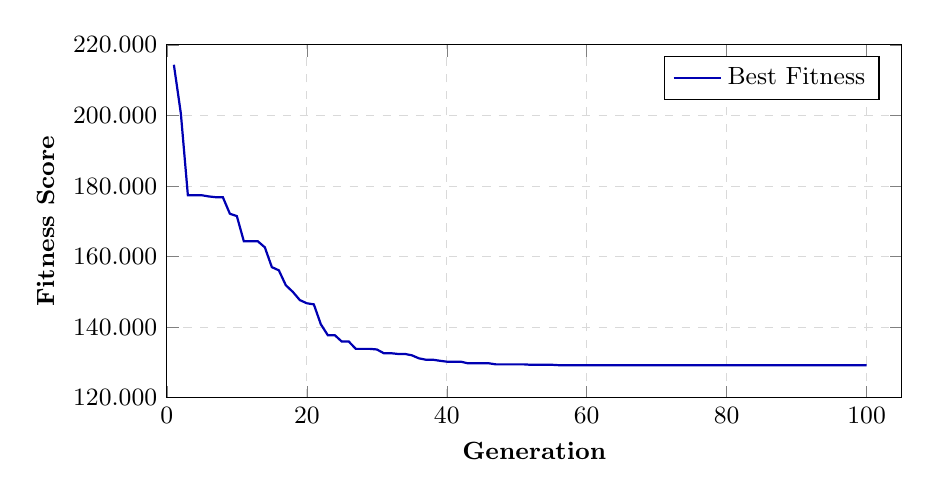
\begin{tikzpicture}
        \begin{axis}[
            width=0.9\textwidth,
            height=0.5\textwidth,
            xlabel={Generation},
            ylabel={Fitness Score},
            grid=major,
            grid style={dashed, gray!30},
            legend pos=north east,
            legend style={font=\small},
            xmin=0, 
            xmax=105,
            ymin=120000, 
            ymax=220000,
            scaled y ticks=false,
            y tick label style={/pgf/number format/.cd, fixed, precision=0, use comma},
            tick label style={font=\small},
            ylabel style={font=\small\bfseries},
            xlabel style={font=\small\bfseries},
        ]
        
        \addplot[blue!70!black, thick, mark=none] coordinates {
            (1, 214378.7) (2, 200547.9) (3, 177389.9) (4, 177389.9) (5, 177389.9)
            (6, 177058.0) (7, 176838.5) (8, 176838.5) (9, 172168.0) (10, 171478.2)
            (11, 164338.8) (12, 164338.8) (13, 164338.8) (14, 162635.2) (15, 157027.3)
            (16, 156113.3) (17, 151883.5) (18, 150009.9) (19, 147682.1) (20, 146779.8)
            (21, 146471.4) (22, 140838.3) (23, 137733.9) (24, 137733.9) (25, 135923.6)
            (26, 135923.6) (27, 133858.6) (28, 133858.6) (29, 133858.6) (30, 133691.4)
            (31, 132631.4) (32, 132631.4) (33, 132424.6) (34, 132424.6) (35, 132044.0)
            (36, 131186.0) (37, 130786.5) (38, 130786.5) (39, 130487.2) (40, 130231.1)
            (41, 130231.1) (42, 130231.1) (43, 129773.1) (44, 129773.1) (45, 129773.1)
            (46, 129773.1) (47, 129467.7) (48, 129467.7) (49, 129467.7) (50, 129467.7)
            (51, 129467.7) (52, 129347.9) (53, 129347.9) (54, 129347.9) (55, 129347.9)
            (56, 129234.4) (57, 129234.4) (58, 129234.4) (59, 129234.4) (60, 129234.4)
            (61, 129234.4) (62, 129234.4) (63, 129234.4) (64, 129234.4) (65, 129234.4)
            (66, 129234.4) (67, 129234.4) (68, 129234.4) (69, 129234.4) (70, 129234.4)
            (71, 129234.4) (72, 129234.4) (73, 129234.4) (74, 129234.4) (75, 129234.4)
            (76, 129234.4) (77, 129234.4) (78, 129234.4) (79, 129234.4) (80, 129234.4)
            (81, 129234.4) (82, 129234.4) (83, 129234.4) (84, 129234.4) (85, 129234.4)
            (86, 129234.4) (87, 129234.4) (88, 129234.4) (89, 129234.4) (90, 129234.4)
            (91, 129234.4) (92, 129234.4) (93, 129234.4) (94, 129234.4) (95, 129234.4)
            (96, 129234.4) (97, 129234.4) (98, 129234.4) (99, 129234.4) (100, 129234.4)
        };
        \addlegendentry{Best Fitness}
        
        \end{axis}
    \end{tikzpicture}
    \caption{Genetic algorithm over 100 generations on Wizard of Oz book}
    \label{fig:convergence_oz}
\end{figure}

Compared to Moby Dick, the Wizard of Oz optimization exhibits faster convergence. 
Table \ref{tab:convergence_phases_oz} shows that the algorithm reaches near-optimal solutions by generation 56, 
after which no further improvements occur for 44 consecutive generations.

\begin{table}[H]
    \centering
    \caption{Phase analysis (Wizard of Oz)}
    \label{tab:convergence_phases_oz}
    \begin{tabularx}{\textwidth}{@{}Xrrrr@{}}
        \toprule
        \textbf{Phase} & \textbf{Generations} & \textbf{Initial Fit.} & \textbf{Final Fit.} & \textbf{Improvement} \\ 
        \midrule
        Exploration  & 1--20  & 214,378.7 & 146,779.8 & 31.5\% \\
        Explotation & 21--56 & 146,779.8 & 129,234.4 & 12.0\% \\
        Convergence  & 57--100 & 129,234.4 & 129,234.4 & 0.0\% \\
        \midrule
        \textbf{Total} & \textbf{1--100} & \textbf{214,378.7} & \textbf{129,234.4} & \textbf{39.7\%} \\
        \bottomrule
    \end{tabularx}
\end{table}


This earlier convergence suggest that simpler texts result in a less complex optimization with fewer local optimals.
Table \ref{tab:convergence_milestones_oz} presents the fitness score at every 10 generations. 


\begin{table}[H]
    \centering
    \caption{Convergence milestones: Best fitness every 10 generations (Wizard of Oz)}
    \label{tab:convergence_milestones_oz}
    \begin{tabular}{@{}rr|rr@{}}
        \toprule
        \textbf{Generation} & \textbf{Best Fitness} & \textbf{Generation} & \textbf{Best Fitness} \\ 
        \midrule
        1  & 214,378.7 & 60 & 129,234.4 \\
        10 & 171,478.2 & 70 & 129,234.4 \\
        20 & 146,779.8 & 80 & 129,234.4 \\
        30 & 133,691.4 & 90 & 129,234.4 \\
        40 & 130,231.1 & 100 & 129,234.4 \\
        50 & 129,467.7 &     &           \\
        \bottomrule
    \end{tabular}
\end{table}

The evolved layout for the Wizard of Oz corpus is presented in Figure \ref{fig:evolved_layout_oz}. 
Notably, this layout differs substantially from the Moby Dick optimization, reflecting the different 
linguistic characteristics of children's literature.
But keeps the same core strategy. It places the vowels at the center row, with frequent consonats, optimizing the high frequency letters,
reducing their fitness cost. And placing the less frequent letters and punctuation across the top and bottom rows to reduce finger movement.


\begin{figure}[H]
    \centering
    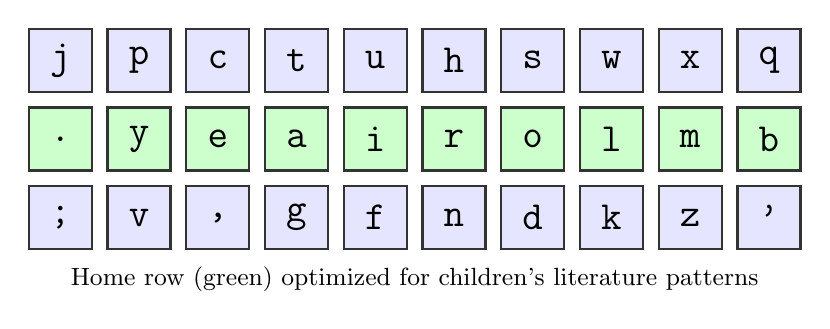
\begin{tikzpicture}[
        key/.style={rectangle, draw=black!80, fill=blue!10, thick, minimum size=0.8cm, font=\Large\ttfamily},
        home/.style={key, fill=green!20},
    ]
    % Row 1
    \node[key] at (0,2) {j}; \node[key] at (1,2) {p}; \node[key] at (2,2) {c}; 
    \node[key] at (3,2) {t}; \node[key] at (4,2) {u}; \node[key] at (5,2) {h}; 
    \node[key] at (6,2) {s}; \node[key] at (7,2) {w}; \node[key] at (8,2) {x}; 
    \node[key] at (9,2) {q};
    
    % Row 2 (Home row - highlighted)
    \node[home] at (0,1) {.}; \node[home] at (1,1) {y}; \node[home] at (2,1) {e}; 
    \node[home] at (3,1) {a}; \node[home] at (4,1) {i}; \node[home] at (5,1) {r}; 
    \node[home] at (6,1) {o}; \node[home] at (7,1) {l}; \node[home] at (8,1) {m}; 
    \node[home] at (9,1) {b};
    
    % Row 3
    \node[key] at (0,0) {;}; \node[key] at (1,0) {v}; \node[key] at (2,0) {,}; 
    \node[key] at (3,0) {g}; \node[key] at (4,0) {f}; \node[key] at (5,0) {n}; 
    \node[key] at (6,0) {d}; \node[key] at (7,0) {k}; \node[key] at (8,0) {z}; 
    \node[key] at (9,0) {'};
    
    \node[below, font=\small] at (4.5, -0.5) {Home row (green) optimized for children's literature patterns};
    \end{tikzpicture}
    \caption{Optimized keyboard layout evolved by genetic algorithm (Wizard of Oz corpus)}
    \label{fig:evolved_layout_oz}
\end{figure}

Table \ref{tab:letter_placement_oz} categorizes the distribution of characters across the three rows. 
The home row contains the majority of vowels and high-frequency consonants, which minimizes finger movement for common sequences. 
The top and bottom rows are reserved for punctuation and less frequent letters, reflecting the algorithm's strategic placement for efficient typing.


\begin{table}[H]
    \centering
    \caption{Letter placement analysis of evolved layout (Wizard of Oz)}
    \label{tab:letter_placement_oz}
    \begin{tabularx}{\textwidth}{@{}l>{\raggedright\arraybackslash}X>{\raggedright\arraybackslash}X@{}}
        \toprule
        \textbf{Row} & \textbf{Characters} & \textbf{Characteristics} \\ 
        \midrule
        Top Row    & j, p, c, t, u, h, s, w, x, q
                  & Mix of common (t, h, s) and rare consonants \\
        Home Row   & ., y, e, a, i, r, o, l, m, b
                  & All five vowels plus frequent consonants \\
        Bottom Row & ;, v, ,, g, f, n, d, k, z, '
                  & Punctuation and moderate-frequency consonants \\
        \bottomrule
    \end{tabularx}
\end{table}


Finally, Table \ref{tab:layout_comparison_oz} compares the fitness scores of the evolved layout with existing layouts. 
The evolved layout significantly outperforms QWERTY, QWERTZ, Dvorak, and Colemak, demonstrating the effectiveness of the genetic algorithm in adapting to the unique characteristics of the text.

\begin{table}[H]
    \centering
    \caption{Fitness comparison of keyboard layouts on Wizard of Oz corpus}
    \label{tab:layout_comparison_oz}
    \begin{tabular}{@{}lrr@{}}
        \toprule
        \textbf{Layout} & \textbf{Fitness Score} & \textbf{Improvement of Evolved GA} \\ 
        \midrule
        QWERTY & 273,549.7 & 52.8\% \\
        QWERTZ & 286,167.2 & 54.8\% \\
        Dvorak & 230,728.3 & 44.0\% \\
        Colemak & 222,474.5 & 41.9\% \\
        \midrule
        \textbf{Evolved GA} & \textbf{129,234.4} & \textbf{--} \\
        \bottomrule
    \end{tabular}
\end{table}

The improvement percentages are remarkably consistent with the Moby Dick results, with only minor variations (±1-2\%). 
This consistency suggests that our fitness function captures the typing patterns and is capable of representing the improvement
in the final individual.

\subsection{Cross comparison of Layouts}

To evaluate the generalization capability of the optimized layouts, a cross-evaluation was performed. 
The layout evolved with the \textit{Moby Dick} corpus was tested on \textit{The Wizard of Oz} text, and vice versa. 
The objective is to determine whether a layout optimized for a text with complex linguistic features (rich and varied vocabulary) 
is more robust than one optimized for a simpler, more repetitive text.

The results of this comparison are presented in Table \ref{tab:cross_comparison}.

\begin{table}[H]
    \centering
    \caption{Cross-comparison of fitness scores for the evolved layouts.}
    \label{tab:cross_comparison}
    \resizebox{\textwidth}{!}{%
    \begin{tabular}{@{}llrc@{}}
        \toprule
        \textbf{Test Corpus} & \textbf{Evolved Layout} & \textbf{Fitness Score} & \textbf{Notes} \\ 
        \midrule
        \multirow{2}{*}{Moby Dick} & Moby Dick & \textbf{799,038.6} & \textit{Baseline (specialized)} \\
                                   & Wizard of Oz & 848,748.9 & Performance of non-specialized layout \\
        \midrule
        \multirow{2}{*}{Wizard of Oz} & Wizard of Oz & \textbf{129,234.4} & \textit{Baseline (specialized)} \\
                                      & Moby Dick & 132,224.5 & Performance of non-specialized layout \\
        \bottomrule
    \end{tabular}%
    }
\end{table}

The results in Table \ref{tab:cross_comparison} show us how the layouts and the algorithm behaved:

\begin{itemize}
    \item \texttt{Confirmed Specialization:} Each layout performed best on its own book. 
    This demonstrates effective \textbf{exploitation}, where the algorithm perfected the best-found layouts by fine-tuning them to 
    the specific letter patterns of each text.

    \item \texttt{Over-specialization of the Simple-Text Layout:} The \textit{Wizard of Oz} layout struggled on the complex text, 
    with a 6.2\% performance drop. The simple book offered a limited field for \textbf{exploration}, leading the algorithm to 
    over-specialize on a narrow solution that lacked flexibility.

    \item \texttt{Robustness of the Complex-Text Layout:} Conversely, the \textit{Moby Dick} layout was very robust, 
    dropping only 2.3\% on the simpler text. The book's rich language provided a better landscape for \textbf{exploration}, 
    allowing the algorithm to discover a more versatile solution before the final \textbf{exploitation} phase, resulting in a 
    more robust layout.

\end{itemize}


\chapter{Simulated Annealing Methodology} \label{chpt:4}

\chapter{Conclusions} \label{chpt:6}
\section{Summary of the developed work}
\section{Achieved objectives}
\section{Future work}

%%%%%%%%%%%%%%%%%%%%%%%%%%%%%%%%%%%%%%%%%%%%%%%%%%%%%%%%%%%%%%%%%%%%%%%%%%%%%%%
%                                BIBLIOGRAPHY                                 %
%%%%%%%%%%%%%%%%%%%%%%%%%%%%%%%%%%%%%%%%%%%%%%%%%%%%%%%%%%%%%%%%%%%%%%%%%%%%%%%

\cleardoublepage
% \bibliographystyle{plain}
% \bibliography{references} % Uncomment if you have a .bib file

%%%%%%%%%%%%%%%%%%%%%%%%%%%%%%%%%%%%%%%%%%%%%%%%%%%%%%%%%%%%%%%%%%%%%%%%%%%%%%%
%                                 APPENDICES                                  %
%%%%%%%%%%%%%%%%%%%%%%%%%%%%%%%%%%%%%%%%%%%%%%%%%%%%%%%%%%%%%%%%%%%%%%%%%%%%%%%

% \appendix
% \chapter{Sustainable Development Goals (SDGs)}
% Appendix content here

%%%%%%%%%%%%%%%%%%%%%%%%%%%%%%%%%%%%%%%%%%%%%%%%%%%%%%%%%%%%%%%%%%%%%%%%%%%%%%%
%                              END OF DOCUMENT                                %
%%%%%%%%%%%%%%%%%%%%%%%%%%%%%%%%%%%%%%%%%%%%%%%%%%%%%%%%%%%%%%%%%%%%%%%%%%%%%%%

\end{document}